% !TeX spellcheck = pt_BR
\documentclass[tese_patricia]{subfiles}
\begin{document}

% ---------------------------------------------------------- 
% Métodos de malhas sobrepostas
% ----------------------------------------------------------
\chapter[Acoplamento Fluido-Estrutura]{Interação Fluido-Estrutura} \label{capitulo:Cap5}
% ----------------------------------------------------------

 O acoplamento entre Fluido e Estrutura proposto nesse trabalho é do tipo particionado forte através da técnica de bloco iterativo. O acoplamento foi resultado do desenvolvimento computacional dos modelos matemáticos apresentados nos capítulos anteriores deste trabalho, ou seja, das equações que descrevem o comportamento do fluido, do \textit{Capítulo 1} e \textit{Capítulo 2}, juntamente com a técnica de decomposição de domínios baseada no método Arlequin para o modelo de fluido apresentada no \textit{Capítulo 4}, e,  também, a metodologia de análise não linear de estruturas de casca pelo método dos elementos finitos posicional vista no \textit{Capítulo 3}.
 
 Nesse contexto, para o acoplamento, utiliza-se a técnica de rastreamento de interface para a malha local do fluido em contato com a estrutura, na qual aplica-se uma descrição Lagrangiana-Euleriana arbitrária, fazendo com que o domínio computacional local possa ser movido independentemente do movimento do fluido. 
 
 No texto a seguir apresentam-se inicialmente as condições de acoplamento que possibilitam a resolução dos problemas da IFE, o tipo de acoplamento utilizado e, por fim, a técnica de movimentação de malhas aplicada.

\section{Condições de acoplamento}

Os problemas de IFE são caracterizados pela interdependência entre o fluido e a estrutura, visto que o comportamento do escoamento depende do formato e do movimento da estrutura, enquanto que o movimento da estrutura e sua deformação dependem das forças do fluido que atuam sobre ela. Matematicamente pode-se dizer que os problemas de IFE são conjuntos de equações e condições de contorno associadas ao fluido e a estrutura que devem ser satisfeitas simultaneamente.

O domínio computacional para a análise de problemas de interação fluido-estrutura (Fig. \ref{fig:dominios}), denominado de $\Omega_{IFE}$, é composto pela união entre os domínios da estrutura $\Omega_E$ e do fluido $\Omega_F$, ou seja, $\Omega_{IFE} = \Omega_F \cup \Omega_E$, com $\Gamma_{IFE}$ o sendo o contorno que define a interface fluido-estrutura.

\begin{figure}[htb!]
	\centering 
	%\vspace{-1em} % Diminui o espaço antes da figura
	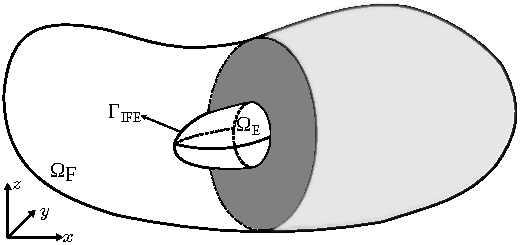
\includegraphics[scale=1.0,trim=0cm 0cm 0cm 0.0cm, clip=true]{Imagens/Cap5/dominio.pdf}	
	\caption{Domínios do Fluido e da Estrutura.}
	\label{fig:dominios}
	%\vspace{-1em} % Diminui o espaço antes da figura
\end{figure}

O domínio computacional não se sobrepõe, por isso, é necessário que em $\Gamma_{IFE}$ existam condições físicas adicionais para se realizar o acoplamento. \citeonline{richter2017fluid} cita que o acoplamento é realizado através de 3 diferentes princípios no contorno $\Gamma_{IFE}$ : condição cinemática, condição dinâmica e condição geométrica.

A condição cinemática refere-se ao fato de que a velocidade do fluido e do sólido na interface devem ser iguais, ou seja:

\begin{align}
\velocityh = \solidVel^h \ \textrm{no contorno} \ \Gamma_{IFE}
\end{align}

A condição dinâmica, preescreve o balanço da tensão normal no contorno, ao que diz respeito à ação e reação, conforme a equação abaixo:

\begin{align}
\mathbf{\sigma}_{E}\mathbf{n}_{E} + \mathbf{\sigma}_{F}\mathbf{n}_{F} = 0 \ \textrm{no contorno} \ \Gamma_{IFE},
\end{align}

\noindent na qual, $\mathbf{\sigma}_{E}$ representa as tensões de Cauchy da estrutura, $\mathbf{\sigma}_{F}$ as tensões de Cauchy no fluido, e $\mathbf{n}_E$ e $\mathbf{n}_F$ representam o vetor normal no contorno $\Gamma_{IFE}$ respectivamente apontando para o fluido e para a estrutura.

Já a condição geométrica está relacionada ao fato que os domínios computacionais $\Omega_E$ da estrutura e $\Omega_F$ do fluido devem sempre coincidir em $\Gamma_{IFE}$, ou seja, não devem existir superposições ou frestas nessa interface.


\section{Técnica de Acoplamento - Bloco-Iterativo}

Nessa seção se apresenta a técnica de acoplamento de Bloco-Iterativo, conforme \citeonline{BazilevsTT:2013}. As equações completas discretizadas da formumação de IFE conduzem a um sistema equações não-lineares que devem ser resolvidas a cada passo de tempo e podem ser representadas da seguinte maneira:

\begin{align}
	\mathbf{N}_{1}\left(\mathbf{d}_{1},\mathbf{d}_{2},\mathbf{d}_{3}\right) = 0,\\
	\mathbf{N}_{2}\left(\mathbf{d}_{1},\mathbf{d}_{2},\mathbf{d}_{3}\right) = 0,\\
	\mathbf{N}_{3}\left(\mathbf{d}_{1},\mathbf{d}_{2},\mathbf{d}_{3}\right) = 0,
\end{align}

\noindent em que $\mathbf{{N}_{1}}$, $\mathbf{{N}_{2}}$ e $\mathbf{{N}_{3}}$ representam as equações que descrevem o fluido, a estrutura e a malha respectivamente, e, $\mathbf{{d}_{1}}$, $\mathbf{{d}_{2}}$, $\mathbf{{d}_{3}}$ são vetores com as variáveis nodais de cada meio. 
A resolução dessas equações através do método de Newton-Raphson conduz ao seguinte sistema linear de equações:

\begin{align}
\mathbf{A_{11}}\mathbf{x_{1}} + \mathbf{A_{12}}\mathbf{x_{2}} + \mathbf{A_{13}}\mathbf{x_{3}} = \mathbf{b_{1}}\\
\mathbf{A_{21}}\mathbf{x_{1}} + \mathbf{A_{22}}\mathbf{x_{2}} + \mathbf{A_{23}}\mathbf{x_{3}} = \mathbf{b_{2}}\\
\mathbf{A_{31}}\mathbf{x_{1}} + \mathbf{A_{32}}\mathbf{x_{2}} + \mathbf{A_{33}}\mathbf{x_{3}} = \mathbf{b_{3}}
\end{align}

\noindent sendo $\mathbf{b_{1}} = - \mathbf{N}_{1}$, $\mathbf{b_{2}} = - \mathbf{N}_{2}$, $\mathbf{b_{3}} = - \mathbf{N}_{3}$. $\mathbf{x_{1}}$, $\mathbf{x_{2}}$ e $\mathbf{x_{3}}$ são os incrementos às soluções $\mathbf{d}_{1}$, $\mathbf{d}_{2}$ e $\mathbf{d}_{3}$ respectivamente e $\mathbf{A_{ij}} = \frac{\partial\mathbf{N}_{i}}{\partial\mathbf{d}_{j}}$. 

Quando se utiliza o acoplamento forte do tipo bloco iterativo, para cada passo de iteração se resolve sequencialmente cada um dos três blocos, conforme apresentado a seguir:


\begin{align}
	\left .\frac{\partial\mathbf{N}_{1}}{\partial\mathbf{d}_{1}}\right|_{\left(\mathbf{d}_{1}^{i},\mathbf{d}_{2}^{i},\mathbf{d}_{3}^{i}\right)} \Delta\mathbf{d}_{1}^{i} = - \mathbf{N}_{1}\left(\mathbf{d}_{1}^{i},\mathbf{d}_{2}^{i},\mathbf{d}_{3}^{i}\right)\\
	\mathbf{d}_{1}^{i+1} =  \mathbf{d}_{1}^{i} + \Delta\mathbf{d}_{1}^{i}	\\
	\left.\frac{\partial\mathbf{N}_{2}}{\partial\mathbf{d}_{2}}\right|_{\left(\mathbf{d}_{1}^{i+1},\mathbf{d}_{2}^{i},\mathbf{d}_{3}^{i}\right)} \Delta\mathbf{d}_{2}^{i} = - \mathbf{N}_{2}\left(\mathbf{d}_{1}^{i+1},\mathbf{d}_{2}^{i},\mathbf{d}_{3}^{i}\right)\\
	\mathbf{d}_{2}^{i+1} =  \mathbf{d}_{2}^{i} + \Delta\mathbf{d}_{2}^{i} \\
	\left.\frac{\partial\mathbf{N}_{3}}{\partial\mathbf{d}_{3}}\right|_{\left(\mathbf{d}_{1}^{i+1},\mathbf{d}_{2}^{i+1},\mathbf{d}_{3}^{i}\right)} \Delta\mathbf{d}_{3}^{i} = - \mathbf{N}_{3}\left(\mathbf{d}_{1}^{i+1},\mathbf{d}_{2}^{i+1},\mathbf{d}_{3}^{i}\right)\\
	\mathbf{d}_{3}^{i+1} =  \mathbf{d}_{3}^{i} + \Delta\mathbf{d}_{3}^{i} 
\end{align}


Nas resoluções de problemas IFE, quando a estrutura é leve, a resposta estrutural torna-se muito sensível para pequenas mudanças nas forças proveninetes do fluido. Para resolver esse problema, utilizou-se a técnica apresentada em \citeonline{Tezduyar:2003d}, onde para corrigir o deslocamento estrutural durante a resolução a matriz de massa em $\mathbf{A_{22}}$ é aumentada. Isso ocorre sem que $\mathbf{b_{1}}$, $\mathbf{b_{2}}$ e $\mathbf{b_{3}}$ sejam alterados, ou seja, sem que ocorra uma mudança nas equações não lineares. Isso faz com que quando a solução por bloco iterativo converge, ela converge sem que seja alterada a massa estrutural real do problema.

\section{Discretizações não coincidentes entre os meios}

Na maioria dos casos a discretização das malhas do fluido e da estrutura são não-coincidentes e podem inclusive ter aproximações matemáticas distintas. Dessa forma, uma metodologia que possibilita a aplicação de condições de contorno em caso de discretizações com nós não coincidentes, é imprescindível. Para isso, uma técnica aplicada em \citeonline {Fernandes:2020} foi utilizada.

Esse procedimento pode ser entendido a partir da Fig. \ref{fig:contornoIFE}. Nele, durante o pré-processamento, cada nó do contorno da estrutura $\mathbf{x_E}$ é projetado sobre o contorno do fluido, e busca-se a coordenada paramétrica relativa a este ponto definida como $\boldsymbol{\xi_{F}}(\mathbf{x_E})$. Da mesma forma, cada nó do contorno do fluido $\mathbf{x_F}$ é projetado sobre o contorno da estrutura, e encontra-se uma coordenada paramétrica equivalente $\boldsymbol{\xi_{E}}(\mathbf{x_F})$. 


\begin{figure}[htb!]
	\centering 
	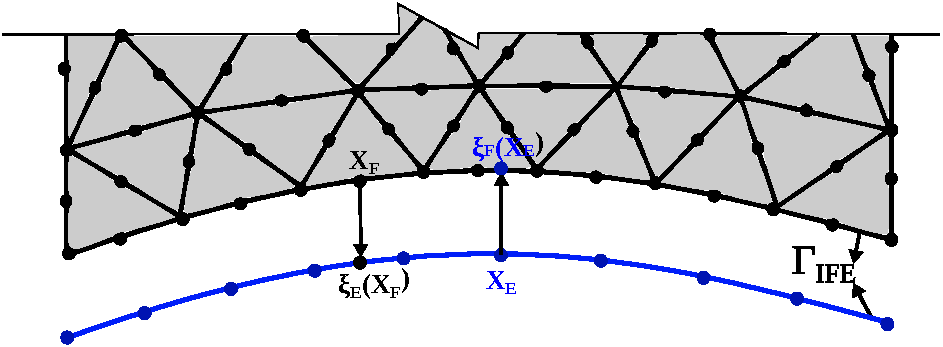
\includegraphics[scale=0.9,trim=0cm 0cm 0cm 0cm, clip=true]{Imagens/Cap5/contornoIFE.pdf}	
	\caption{Contorno IFE}
	\label{fig:contornoIFE}
\end{figure}

Dessa forma, as informações que serão transmitidas ao fluido pela estrutura são interpoladas na malha da estrutura em cada uma das coordenadas paramétricas que possuem um nó equivalente na malha de fluido, e após isso aplicadas a este nó. O equivalente ocorre quando os dados são provenientes do fluido e serão transmitidos a estrutura.

\section{Movimentação da Malha}

Nos métodos de malhas adaptadas, à medida em que a interface $\Gamma_{IFE}$ se move, a malha do fluido deve mover-se para ajustar-se ao novo formado e se adaptar à estrutura. Nessa metodologia demanda-se maior controle da resolução da malha próxima a interface dos meios fluidos e sólidos, possibilitando o uso de uma melhor discretização para representar os efeitos de camada limite, e como consequência, a obtenção de soluções mais acuradas nessas regiões críticas.

Para possibilitar esse controle, neste trabalho será utilizada a técnica de movimentação de malhas introduzida em \citeonline{TezduyarBSJ:1992f} e \citeonline{TezduyarABJ:1993} conhecida como MJBS (\textit{Mesh-Jacobian Based Stiffening}).

O movimento da malha é determinado usando um problema da elasticidade de Dirichlet fictício, descrito como:

\begin{align}
	\int_{\domaintt} \straintensor \left(\testfunction\right) : \stresstensor \left(\displacementmesh - \displacementmesh_{\tilde{t}}\right) d\domaintt = 0,
	\label{eq:elasticityequation}
\end{align}

\noindent na qual $\straintensor$ e $\stresstensor$ representam o tensor de deformação linear infinitesimal e o tensor de tensões de Cauchy respectivamente. $\testfunction$ é a função peso respectiva ao deslocamento da malha  $\displacementmesh$, medido a partir de uma configuração de referência até a configuração atual $\currentcoordinates$ e 
$\displacementmesh_{\tilde{t}}$ representa o deslocamento da configuração de referência até a malha no tempo ${\tilde{t}}$, ou $\currentcoordinates_{\tilde{t}}$. 
A escolha para ${\tilde{t}}$ é geralmente ${\tilde{t}} = {t_{n}}$ quando se calcula a configuração da malha no tempo ${t_{n+1}}$ (ver \citeonline{Tononetal:2021} para maiores detalhes). O índice $h$ refere-se à discretização das variáveis por uma aproximação matemática em elementos finitos ou isogeométrica.

O tensor de tensões é calculado através da seguinte relação:

\begin{align}
	\stresstensor(\disp)
	&=
	\frac{E}{1+\poisonsRatio}
	\left(
	\frac{\poisonsRatio}{(1 - 2 \poisonsRatio)}
	\trace\left(\straintensor(\disp)\right)\unittensor
	+
	\straintensor(\disp)
	\right)
\end{align}

\noindent com $E$ e $\poisonsRatio$ o módulo de Elasticidade e o coeficiente de Poisson respectivamente.

Para fazer com que na deformação da malha se leve em conta o tamanho dos elementos, enrijecendo os menores mais do que os maiores, no método MJBS a equação da elasticidade fica descrita ao final como:

\begin{align}
	\int_{\domaintt} \straintensor \left(\testfunction\right) : \stresstensor \left(\displacementmesh- \displacementmesh_{\tilde{t}}\right) \left(\frac{J_M}{\left({J_M}\right)_0}\right)^{-\chi} d\domaintt = 0, 
	\label{eq:MJBS}
\end{align}

\noindent onde $J_M$ é o Jacobiano da malha, $(J_M)_0$ é um parâmetro livre e $\chi$ determina a ordem pela qual os elementos menores serão enrijecidos mais do que os maiores.  $\chi$ é adotado correntemente como 1. E o Jacobiano da malha calculado da forma que se segue:

\begin{align}
	J_M = det\left(\frac{\partial\currentcoordinates_{\tilde{t}}}{\partial\adimensionalcoordinates}\right), 
	\label{eq:3}
\end{align}

\noindent onde $\adimensionalcoordinates$ são as coordenadas paramétricas do elemento.


\section{Cavidade com fundo flexível - 2D}

\begin{figure}[htb!]
	\centering 
	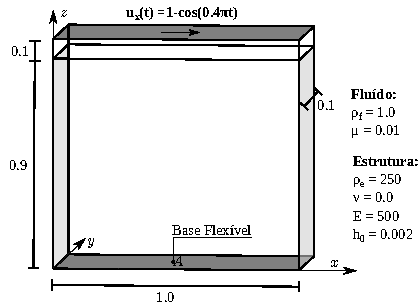
\includegraphics[scale=1.3,trim=0cm 0cm 0cm 0cm, clip=true]{Imagens/Cap5/cav2d.pdf}	
	\caption{Geometria Cavidade Fundo Flexível 2D}
	\label{fig:cavidadeFF2d}
\end{figure}
\section{Cavidade com fundo flexível - 3D}

\begin{figure}[htb!]
	\centering 
	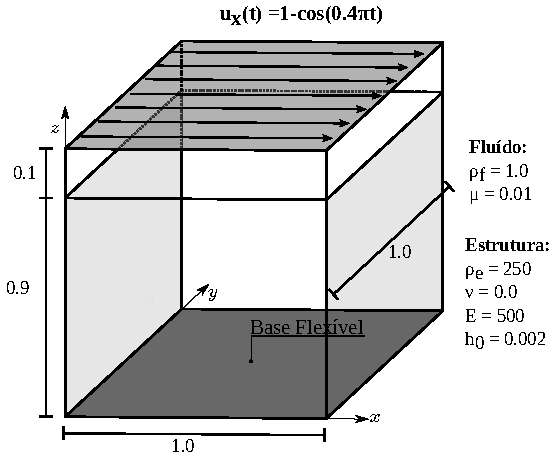
\includegraphics[scale=0.9,trim=0cm 0cm 0cm 0cm, clip=true]{Imagens/Cap5/cav3d.pdf}	
	\caption{Geometria Cavidade Fundo Flexível 3D}
	\label{fig:cavidadeFF3d}
\end{figure}

\end{document}
